\documentclass[a4paper]{article}

\usepackage[utf8]{inputenc}
\usepackage[T1]{fontenc}
\usepackage{textcomp}
\usepackage{listings}
\usepackage{lmodern}
\usepackage{amsfonts}
\usepackage{marvosym}
\usepackage{titling}
\usepackage{lipsum}
\usepackage[left=1in, right=1in, bottom=1in, top=1in]{geometry}
\usepackage{mathtools}
\usepackage{amsthm}
\usepackage{tcolorbox}
\usepackage{hyperref}
\usepackage{xcolor}
\usepackage{graphicx}
\usepackage{makeidx}
\usepackage{tikz}
\usepackage{cases}
\usepackage{apacite}
\usepackage{tkz-berge}
\usepackage{lastpage}
\usepackage{fancyhdr}
\pagestyle{fancy} 
\usepackage{url}
\usepackage{tgtermes}
\usepackage{sectsty}
\usepackage{subcaption}
\usepackage{setspace}
\usepackage{float}
\usepackage{amsmath, amssymb}
\rhead{Page~\thepage~of~\pageref{LastPage}}
\cfoot{\hline \vspace{3mm} Written by Cem Yilmaz}

% figure support
\usepackage{import}
\usepackage{xifthen}
\pdfminorversion=7
\usepackage{pdfpages}
\usepackage{transparent}
\newcommand{\incfig}[2][1]{%
	\def\svgwidth{#1\columnwidth}
	\import{./figures/}{#2.pdf_tex}
}

%mathstyling
\theoremstyle{plain}
\newtheorem{thm}{Theorem}[section]
\newtheorem{lem}[thm]{Lemma}
\newtheorem{prop}[thm]{Proposition}
\newtheorem*{cor}{Corollary}

\theoremstyle{definition}
\newtheorem{defn}{Definition}[section]
\newtheorem{conj}{Conjecture}[section]
\newtheorem{exmp}{Example}[section]
\newtheorem{axiom}{Axiom}
\theoremstyle{remark}
\newtheorem*{rem}{Remark}
\newtheorem*{note}{Note}

\pdfsuppresswarningpagegroup=1

\begin{document}
\begin{titlepage}
\begin{center}
\large
University of Warwick \\
Department of Computer Science \\

\huge
\vspace{50mm}
\rule{\linewidth}{0.5pt}\\
CS130\\
\vspace{5mm}
\Large
Mathematics for Computer Scientists I
\rule{\linewidth}{0.5pt}
\vspace{5mm}
\begin{figure}[H]
	\centering
	
\includegraphics[width=0.4\textwidth]{crest_black.eps}
	\label{fig:}
\end{figure}
\vspace{37mm}
Cem Yilmaz\\
\today
\end{center}
\end{titlepage}

\tableofcontents 
\newpage 
\section{Induction} 
\subsection{Inductive definition} 
Inductive definitions are such that there is an initial case followed by an infinite case. For example: $a_0=0$ ad $a_{n+1} = 2a_n+1$ where $n \in \mathbb{N}$.  
\subsection{Inductive proof} 
Inductive proof is used similarly to what an inductive definition would be, it would begin with a first case and then work until infinity.  
\section{Functions} 
\begin{tcolorbox}[colback=black!3!white,colframe=black!60!white,title=\begin{defn}Function Notation \label{Function Notation}\end{defn}] 
The notation $f:X \to Y$ reads as mapping every element of $X$ to an ambiguous element of the set $Y$. In other words, $f$ such that $X$ maps to  $Y$. If we consider some number $x$ such that $x \in X$, we can consider the mapping \\ \begin{align*} x \mapsto x^2-3 \end{align*} The set of $X$ and $Y$ in $f: X \to  Y$ is called domain and range. However, codomain is defined to be the numbers in range which do exist in set y, but are not necessarily mapped from the set $X$. \\ 
Note: we use the notation $\to $ to denote mapping from set to set and the notation $\mapsto$ when we talk about variables in $X$.  
\end{tcolorbox} 
\begin{tcolorbox}[colback=black!3!white,colframe=black!60!white,title=\begin{defn}Definition of a function\label{Definition}\end{defn}] 
A function is defined as something that maps \emph{all} elements in $X$ to \emph{an} element in $Y$.  
\begin{figure}[H] 
	\centering 
	\incfig{function} 
	\caption{$X$ set mapping to $Y$ set. $x$ maps to $y$.} 
	\label{fig:function} 
\end{figure} 
\end{tcolorbox} 
\begin{tcolorbox}[colback=black!3!white,colframe=black!60!white,title=\begin{exmp}Question 1 \label{Question 1}\end{exmp}] 
Which are functions that are $f:\mathbb{R} \to  \mathbb{R}$?  
\begin{enumerate} 
	\item $f_1(x)=\frac{1}{x}$ 
	\item $f_2(x)=\sqrt{x} $ 
	\item $f_3(x)=\pm\sqrt{x^2+1} $ 
\end{enumerate} 
\begin{align} 
	\text{$f_1$ is not a function as $f\left( 0 \right)$ is undefined.} \\ 
	\text{$f_2$ is not a function as $x<0$ is undefined.} \\ 
	\text{$f_3$ is not a function as when mapping a single $x$ value, it maps into to two values ($\pm\sqrt{a} $ )}\\
	\text{therefore it is actually $f:\mathbb{R}\to \mathbb{R}^2$.} 
\end{align} 
It is okay that multiple elements in $X$ map into the same element in $Y$. However, it is not okay if a single $X$ element maps to multiple $Y$ elements.  
		\end{tcolorbox} 
		\subsection{Relationship Functions} 
		\begin{tcolorbox}[colback=black!3!white,colframe=black!60!white,title=\begin{defn}Relation \label{Relation}\end{defn}] 
		A relation $R \subseteq X \times Y$ is a function if for every $x \in X$ there is a unique $y \in Y$ such that $xRy$. If we denote the function by $f$, then for every  $x \in X$, the unique $y \in Y$ s.t. $xRy$ is denoted $f(x)$. In other words, $f(x)$ is the unique $y$ (image) for an $x$.  $x$ is also the pre-image of $y$.  
	\end{tcolorbox} 
	\subsection{Pre-image}
	\begin{tcolorbox}[colback=black!3!white,colframe=black!60!white,title=\begin{defn}Pre-image \label{Pre-image}\end{defn}]
	Let $f: A \to B$ be a map between sets $A$ and $B$. The the preimage of $Y$ under $f$ is denoted by $f^{-1}(Y)$, and is the set of all elements of $A$ that map to elements in $Y$ under $f$. Not to confuse with the inverse a function. Note that the complete pre-image of a function is always a set. A more general difference can be seen if we consider elements  $a,  \alpha \in A$, $a \neq \alpha : a \mapsto y \land \alpha \mapsto y$. In this case, the preimage would contain both $a$ and $\alpha$, but it is not a function. In a function, we would require to either have $a$ or $\alpha$.
	\begin{align}
		f^{-1}(Y) = \{ a \in A : f(a) \in Y \}
	\end{align}
\end{tcolorbox}
\subsection{Failure to be a function}
Remember that
\begin{enumerate}
	\item Every $x \in X$ must be mapped.
	\item You cannot have $x$ map into more than one.
\end{enumerate}
\subsection{Composition of functions}
Recall that $R \subseteq A \times B$ and $Q \subseteq B \times C$, then $R \circ Q$, the composition of two relations.
\begin{tcolorbox}[colback=black!3!white,colframe=black!60!white,title=\begin{thm}Function Composition \label{Function Composition}\end{thm}]
If $f:X \to  Y$ and $g:Y \to Z$, the relation $f \circ g \subseteq X \times Z$ and is a function.
\end{tcolorbox}
\subsection{Properties of functions}
\begin{tcolorbox}[colback=black!3!white,colframe=black!60!white,title=\begin{defn}Injectivity \label{Injectivity}\end{defn}]
A function $f:X \to Y$ is injective if it is one to one. That is, for every $x \in X$ maps to a unique  $y \in Y$. 
\end{tcolorbox}
\begin{tcolorbox}[colback=black!3!white,colframe=black!60!white,title=\begin{defn}Surjectivity \label{Surjectivity}\end{defn}]
A function $f:X \to Y$ is surjective if every value for every $y \in Y$, $\exists x \in X$ such that $f(x)=y$. That is, every $y$ is matched.
\end{tcolorbox}
\begin{tcolorbox}[colback=black!3!white,colframe=black!60!white,title=\begin{defn}Bijectivity \label{Bijectivity}\end{defn}]
A function $f:X \to Y$ is bijective if it is both injective and surjective. 
\end{tcolorbox}
\begin{tcolorbox}[colback=black!3!white,colframe=black!60!white,title=\begin{thm}Inverse bijectivity \label{Inverse bijectivity}\end{thm}]
A function $f:X \to Y$ is bijective if and only if the inverse relation $f^{-1} \subseteq Y \times X$ is a function.
\end{tcolorbox}
\section{Set Theory}
In set builder notation, the set that is described as
\begin{align*}
	E = \{2n : n \in \mathbb{Z}\}
\end{align*}
Is read as, from the brackets "the set of all things of form", whilst the colon describes "such that". Hence, the expression reads as "$E$ equals the set of all things of form 2n, such that $n$ takes on all values in $\mathbb{Z}$., therefore the general rule is the following:
\begin{tcolorbox}[colback=black!3!white,colframe=black!60!white,title=\begin{defn}Set Builder Notation \label{Set Builder Notation}\end{defn}]
General rule for set-builder notation is, for an example set of $X$,
\begin{align}
	X = \{\text{expression}:\text{rule}\}
\end{align}
Similarly, the cardinality of a set is expressed by
\begin{align}
	|X|
\end{align}
This counts the number of elements in a set.
\end{tcolorbox}
\subsection{Cardinality of two sets}
\begin{tcolorbox}[colback=black!3!white,colframe=black!60!white,title=\begin{defn}Equinumerosity \label{Equinumerosity}\end{defn}]
Sets $A$ and $B$ are equinumerous if there is a bijection $f: A \to B$. This is denoted as $A \cong B$. In other words, they're isomorphic. 
\end{tcolorbox}
However, how would we define the cardinalities of $\mathbb{N}$, $\mathbb{R}$, $\mathbb{Q}$ etc.?
Notice the following:
\begin{align*}
	A &\cong A, \; \forall A; \\
	A &\cong B \implies B \cong A, \; \forall A,B; \\
	A &\cong B, B \cong C \implies A \cong C, \; \forall A,B,C
\end{align*}
Notice that this is in fact an equivalence relation.
\begin{tcolorbox}[colback=black!3!white,colframe=black!60!white,title=\begin{defn}Countability \label{Countability}\end{defn}]
Consider the set
\begin{align*}
	F_i = \{ x \in \mathbb{N} : x < n \}
\end{align*}
Then,
\begin{enumerate}
	\item It is labelled "finite" if $S \cong F_i$ for some $i$;
	\item It is labelled "countably infinite: if $S \cong \mathbb{N}$;
	\item It is labelled as "countable" if it's finite or countably infinite;
	\item It is labelled as "uncountable" if it's not countable.
\end{enumerate}
\end{tcolorbox}

\begin{tcolorbox}[colback=black!3!white,colframe=black!60!white,title=\begin{exmp}Examples \label{Examples}\end{exmp}]
Consider $\mathbb{N} \backslash \{ 0 \} \cong \mathbb{N}$
\begin{align}
	f : \mathbb{N} \to \mathbb{N} \backslash \{ 0\}
\end{align}
For $f(x) = x + 1,$ where $x \in \mathbb{N}$. Hence, it is countably infinite. \\

Consider $E = \{ x \in \mathbb{N}: \text{ x is even } \cong \mathbb{N}$, then
	\begin{align}
		f: \mathbb{N} \to  E 
	\end{align}
	Lastly, $\mathbb{Z} \cong \mathbb{N}$, where $f: \mathbb{N} \to  \mathbb{Z}$.
	Consider
\end{tcolorbox}
\begin{tcolorbox}[colback=black!3!white,colframe=black!60!white,title=\begin{thm}$\mathbb{N}^2 \cong \mathbb{N}$ \label{finite countability of nsquared}\end{thm}]
This is countably infinite.
\begin{figure}[H]
	\centering
	\incfig{nsquar}
	\caption{$\mathbb{N}^2$ graph and mapping}
	\label{fig:nsquar}
\end{figure}
Notice that, if we were to pair every $(0,\ldots)$ to $\mathbb{N}$, we would have issue with the fact that the column is infinite. Same logic applies to rows. Therefore, we work diagonally instead as the diagram above
\end{tcolorbox}
\begin{tcolorbox}[colback=black!3!white,colframe=black!60!white,title=\begin{thm}Powerset Isomorphism \label{Powerset Isomorphism}\end{thm}]
If $S$ is a set, then $S \not\cong 2^{S}$. 
\begin{proof}
	Assume $\exists f : S \to 2^{S}$ is a bijection.
	Let $A = \{ x \in S : x \not\in f(x)\}$.
	It follows that $A \subseteq S$ and $A \in 2^{S}$. And we know, for $A \in 2^{S}$, $\exists y \in S : f(y) = A$. Consider two cases
	\begin{enumerate}
		\item $y \in A \implies y \not\in f(y) = A$. That is, if we know that $y$ is in $A$, we must have the condition we set for $A$ but get $y \not\in f(y) =A$ instead.
		\item $y \not\in A \implies y \in f(y) = A$. But this is also a contradiction, considering that it is not in $y$, but still its equal to $A$.
	\end{enumerate}
\end{proof}
\end{tcolorbox}
\subsection{Cartesian Product}
\begin{tcolorbox}[colback=black!3!white,colframe=black!60!white,title=\begin{defn}Cartesian Product \label{Cartesian Product}\end{defn}]
The cartesian product of two sets $A$ and $B$ is another set, denoted as $A \times B$.
\begin{align}
	A \times B = \{(a,b):a \in A, b \in B\}
\end{align}
\end{tcolorbox}
\begin{tcolorbox}[colback=black!3!white,colframe=black!60!white,title=\begin{exmp}Cartesian Product Example \label{Cartesian Product Example}\end{exmp}]
Consider sets $A$ and $B$ where $A=\{a,b,c\}$ and $B=\{x,y,z\}$, then $A \times B$
\begin{align}
	A \times B = \{(a,x),(a,y),(a,z),(b,x),(b,y),(b,z),(c,x),(c,y),(c,z)\}
\end{align}
In other words, you ensure that the pair of a single element in one of the sets has all possible combinations with other sets. These pair of numbers are called ordered pairs. The cardinality also follows that
\begin{align}
	\mid A \times B \mid =  \mid A \mid \times  \mid B \mid 
\end{align}
However, for this to be true, $A,B$ must be finite.
\end{tcolorbox}
It also an interesting fact that $\mathbb{R}^{2}$ is $\mathbb{R} \times \mathbb{R}$, which denotes two coordinates $(x,y)$ ! Another thing to note that $\mathbb{R} \times \mathbb{Z} \times \mathbb{N} \neq \mathbb{R} \times (\mathbb{Z} \times \mathbb{N})$ since the former is $\{(x,y,z): x \in \mathbb{R}, y \in \mathbb{Z}, z \in \mathbb{N}\}$ whereas the latter $\{(x,(y,z)):x \in \mathbb{R}, (y,z) \in \mathbb{Z}\times \mathbb{N}\}$
\subsection{Subsets}
\begin{tcolorbox}[colback=black!3!white,colframe=black!60!white,title=\begin{defn}Subset \label{Subset}\end{defn}]
For sets $A,B$, $A$ is a subset of $B$ iff every element in $A$ is also an element of $B$.
\begin{align}
	A \subseteq B
\end{align}
Similarly, it is not a subset iff there is at least 1 element that is not shared.
\end{tcolorbox}
\begin{tcolorbox}[colback=black!3!white,colframe=black!60!white,title=\begin{defn}$\varnothing \subseteq A$ \label{varnothing subseteq A}\end{defn}]
For any set $A$, the empty set is always a subset. By definition \ref{Subset}, we know that something is not a subset when there is at least one element of the other subset that is not shared. However, empty set has no elements, and thus it is automatically a subset. 
\end{tcolorbox}
\begin{tcolorbox}[colback=black!3!white,colframe=black!60!white,title=\begin{thm}$2^n$ Subsets \label{$2^n$ Subsets}\end{thm}]
If a finite set has $n$ elements, then it has $2^n$ subsets.
\begin{proof}
	For every element present, we have $2$ selections to go through, add the element or not. Then, for this decision, we can add another choice of selections for the next element. We continue this until we have covered all $n$ elements.
\end{proof}
\end{tcolorbox}

\begin{figure}[H]
	\centering
	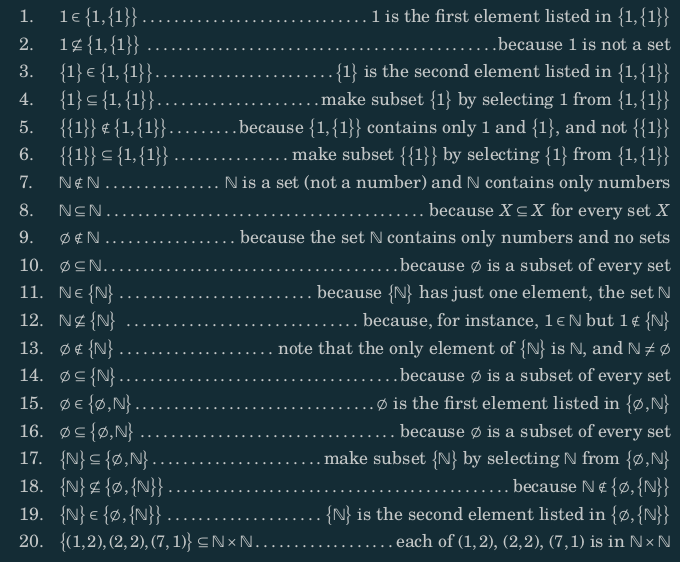
\includegraphics[width=0.8\textwidth]{figures/subsets.png}
	\caption{Rules of "in" and "subsets"}
	\label{fig:figures-subsets-png}
\end{figure}
\subsection{Set Operators}
\begin{align*}
	A \cup B &= \{ x : x \in A \text{ and } x \in B \} \\
	A \cap B &= \{ x : x \in A \text{ and } x \in B \}\\
	A \backslash B &= \{ x: x \in A \text{ and } x \notin B \}\\
	A \triangle B &= (B \backslash A ) \cup (A \backslash B) &= A \cup B \backslash A \cap B \\
	\overline{A} &= S \backslash A &\text{Where $A \subseteq S$}
\end{align*}
\subsection{Power Set}
\begin{tcolorbox}[colback=black!3!white,colframe=black!60!white,title=\begin{defn}Power Set \label{Power Set}\end{defn}]
The power set is defined to be collection of all subsets of some set.
\begin{align}
	\mathbb{P}\left( \{a\} \right) = \{\varnothing, \{a\}\}
\end{align}
\end{tcolorbox}
\section{Boolean Logic}
\subsection{Logic of Propositions}
\begin{tcolorbox}[colback=black!3!white,colframe=black!60!white,title=\begin{defn}Atomic Propositions \label{Atomic Propositions}\end{defn}]
This propositions consist of simple statements $p$.
\begin{align}
	p_1,p_2,q
\end{align}

\end{tcolorbox}
\begin{tcolorbox}[colback=black!3!white,colframe=black!60!white,title=\begin{defn}Compound Propositions \label{Compound Propositions}\end{defn}]
Compound propositions consists of composite of propositions e.g.
\begin{align}
	p \land q
\end{align}
\end{tcolorbox}
\subsection{Logical Statements}
In this section, we will show the logical propositions that are used in computer science.
Note that every logical function is of the kind
\begin{align*}
	F:B^{n}\to B
\end{align*}
where $n \in \mathbb{Z}^{+}$ and $B \in \{T,F\}$
\subsubsection{NOT}
A "not" statement (negation) would imply that it is the opposite of something. For example, if we state that statement $A$ is true, then not statement $A$ would be false. It is denoted by the symbol $\neg$. The truth table is as follows:
\begin{table}[H]
	\centering
	\caption{NOT Statement}
	\label{tab:NOT}
	\begin{tabular}{cc}
		\hline
		Value 1 & Output \\
		\hline
		T & F \\
		F & T \\
		\hline
	\end{tabular}
\end{table}
\subsubsection{AND}
An "and" (conjunction) statement states that $A$ and $B$ can only be true when both are true. This is denoted by the symbol $\land$. The truth table is as follows:
\begin{table}[H]
	\centering
	\caption{AND Statement}
	\label{tab:AND}
	\begin{tabular}{ccc}
		\hline
		Value 1 & Value 2 & Output \\
		\hline
		T & T & T  \\
		T & F & F \\
		F & T & F \\
		F & F & F \\
		\hline
	\end{tabular}
\end{table}
\subsubsection{OR}
An "or" statement (disjunction) states that $A$ and $B$ can only provide a true output as long as one of them is true. This symbol is donated by $\lor$. The truth table is as follows:
\begin{table}[H]
	\centering
	\caption{OR Statement}
	\label{tab:OR}
	\begin{tabular}{ccc}
		\hline
		Value 1 & Value 2 & Output \\
		\hline
		T & T & T \\
		T & F & T \\
		F & T & T \\
		F & F & F \\
		\hline
	\end{tabular}
\end{table}
\subsubsection{XOR}
A "XOR" (Exclusive OR) states that $A$ and $B$ can only provide a true statement as long as one of them true, excluding the case where both are true. This symbol is donated by $\oplus$. The truth able is as follows:
\begin{table}[H]
	\centering
	\caption{XOR Statement}
	\label{tab:XOR}
	\begin{tabular}{ccc}
		\hline
		Value 1 & Value 2  & Output \\
		\hline
		T & T & F \\
		T & F & T \\
		F & T & T \\
		F & F & F \\
		\hline
	\end{tabular}
\end{table}
\newpage
\subsubsection{Equivalence}
An "Equivalence" (Otherwise known as biconditional, iff) states that as long as both $A$ and $B$ have the same binary outputs, then the output is true. It can also be used for more complex logical statements to state that they're the same. This symbol is denoted by  $\equiv$ or $\leftrightarrow$. The truth table is as follows:
\begin{table}[H]
	\centering
	\caption{Equivalence Statement}
	\label{tab:Equivalence}
	\begin{tabular}{ccc}
		\hline
		Value 1 & Value 2 & Output \\
		\hline
		T & T & T \\
		T & F & F \\
		F & T & F \\
		F & F & T \\
		\hline
	\end{tabular}
\end{table}
Notice that this is actually $\neg\left( A \oplus B \right) $.
\subsubsection{Material Conditional \label{mat}}
A "Material Conditional" states that if $A$, then $ B$. There are many ways looking at this statement, such as $B$ only if $A$. What this implies is that if $B$ is true, we know that $A$ must be true. However, if $B$ is false, then we are given no information on $A$, it could be true or false. This symbol is denoted by $\to $. The truth table is as follows:
\begin{table}[H]
	\centering
	\caption{Material Conditional Statement}
	\label{tab:Material Conditional}
	\begin{tabular}{ccc}
		\hline
		Value 1 & Value 2  & Output \\
		\hline
		T & T & T \\
		T & F & F \\
		F & T & T \\
		F & F & T \\
		\hline
	\end{tabular}
\end{table}
Notice that $A \to B = \neg A \lor B$
\subsubsection{Necessity}
Necessity for two statements $P$ and $Q$, for the material equivalence relation $P \implies Q$, would read as "$Q$ is necessary for $P$ ". That is, it is necessary that $Q$ is true for $P$ to be true.
\subsubsection{Sufficiency}
Sufficiency for two statements $P$ and $Q$, for the material equivalence relation $P \impliedby Q$ would be read as "$Q$ is sufficient for $P$". That is, because $Q$ being true always implies $P$ being true, but $P$ not being true does not imply $Q$ is not true. Finally, indeed, one could say $P$ is necessary and sufficient for $Q$, which would give $P \iff Q$.
\subsubsection{Associativity}
Associativity is defined to be that order does not matter in an equation. In boolean logic, it follows that OR statements and AND statements are associative, that is
\begin{align*}
	A \land B \land C \iff (A \land B) \land C \iff A \land (B \land C)\\
	A \lor B \lor C \iff \left( A \lor B \right) \lor C \iff A \lor \left( B \lor C \right) 
\end{align*}
\subsubsection{Commutativity}
Commutativity is defined to show that order does not matter if you switch your variables around.
\begin{align*}
	A \land B \iff B \land A \\
	A \lor B \iff B \lor A
\end{align*}
\subsubsection{Tautology}
\begin{tcolorbox}[colback=black!3!white,colframe=black!60!white,title=\begin{defn}Tautology \label{Tautology}\end{defn}]
Tautology is a statement that is true in all circumstances. That is, it can be done using an either or statement in such way that it cannot be false. For example, the dog is brown or the dog is not brown is a tautology.
\end{tcolorbox}
\subsubsection{Logical Identities}
The following are logical identities:
\[
	\begin{matrix*}[1]
&x \lor F \equiv x &\text{Identity} & x \land T \equiv x\\
&x \lor x \equiv x & \text{Idempotence} & x \land x \equiv x\\
&\neg\left( x \lor y \right) \equiv \neg x \land \neg y & \text{De Morgan's Laws} & \neg \left( x \land y \right) \equiv \neg x \lor \neg y\\
&x \lor \left( x \land y \right) \equiv x & \text{Absorption} & x \land \left( x \lor y \right) \equiv x\\
& x \land \left( y \lor z \right) \equiv (x \land y) \lor \left( x \land z \right) & \text{Distributivity} & x \lor (y \land z) \equiv (x \lor y) \land (x \lor z)\\
& x \lor T \equiv T & \text{Annihilation} & x \land F \equiv F
	\end{matrix*}
\]
There are also identities in which
\begin{align*}
	x \land (\neg x \lor y) \equiv x \land y \\
	x \lor (\neg x \land y ) \equiv x \lor y
\end{align*}
\begin{proof}
	Proof of absorption and equivalence of the absorptions. We begin with the left equation.
	\begin{align*}
		&x \lor (x \land y)\\
		= &\left( x \land T \right) \lor \left( x \land y \right) \\
		= & x \land (T \lor y)\\
		= & x \land T\\
		= & x
	\end{align*}
	Now the right equation
	\begin{align*}
		&x \land (x \lor y)\\
		= &(x \lor F) \land \left( x \lor y \right) \\
		= &x \lor (y \land F)\\
		= &x \lor F\\
		= & x
	\end{align*}
	We show equivalence
	\begin{align*}
		&x \lor \left( x \land y \right) \\
		= & \left( x \lor x \right) \land (x \lor y)\\
		= & x \land (x \lor y)
	\end{align*}
	The other way around
	\begin{align*}
		&x \land \left( x \lor y \right)\\ 
		=&(x \land x) \lor (x \land y)\\
		=&x \lor (x \land y)
	\end{align*}
\end{proof}
\subsubsection{Order of operations}
Listed from most important by ascending order.
\begin{enumerate}
	\item NOT
	\item AND
	\item OR
\end{enumerate}
\subsubsection{Isomorphism}
$\langle T,F,\land,\lor,\neg \rangle$ is isomorphic to $\langle 1,0,min,max,\overline{\phantom{r}} \rangle$ (See Equinumerosity)
\subsection{Different Negations}
\subsubsection{Converse}
This is a special case of the material conditional. $B \to  A$ is called the converse of $A \to  B$.
\subsubsection{Contrapositive}
This is also a special case of the material conditional. $\neg B  \to  \neg A$ is called the contrapositive of $A \to B$. A special property of the contrapositive is that $\neg B \to  \neg A$ shares the same truth values as $A \to B$. This is because the statement is false only when $\neg A$ is false and $\neg B$ is true. That is, originally, $A$ must be true and $B$ must be false.
\subsubsection{Inverse}
Similarly, a special of the material conditional. $\neg A \to \neg B$ is called the inverse of $A \to  B$.
\subsubsection{English Examples}
\begin{tcolorbox}[colback=black!3!white,colframe=black!60!white,title=\begin{exmp}English Example \label{English Example}\end{exmp}]
Let us consider the following statement: ⏎
\begin{center}
	If it is my birthday, I get cake
\end{center} ⏎
The converse of this statement would be "If I get cake, then it is my birthday". ⏎

The contrapositive of this statement would be "If I do not get cake, then it is not my birthday".     ⏎

The inverse would be "If it is not my birthday, then I do not get cake". ⏎ 

Notice that, only the contrapositive of this statement shares the original truth value. That is,  we know that for all birthdays, we get cake, and it is impossible to have an instance that when we do get a cake, it cannot be our birthday (thus false). We are not given any information on when it is not birthday, thus we take all cases when it is not birthday as true. ⏎

The contrapositive statement, on the other hand, works similarly. We know that for all days we do not get cake, then it is not our birthday. However, we cannot have an instance where we do not get cake and it is our birthday (false). We are not given information as to when we do get cake, thus we take all such instances as true.
\begin{align*}
	\forall Birthday \subseteq Cake \iff Cake' \cap Birthday = \varnothing
\end{align*}
\end{tcolorbox}

\begin{tcolorbox}[colback=black!3!white,colframe=black!60!white,title=\begin{exmp}Riemann Hypothesis Statement \label{Riemann Hypothesis Statement}\end{exmp}]
If the research student is to prove the Riemann hypothesis he must be either very clever or else have some luck. If he is not very clever he will not be able to understand number theory. He will fail to finish his thesis only if he has no luck. Therefore, if he proves the Riemann hypothesis, either he understand number theory or he will finish his thesis.\\
The proposition variables here are as follows:
                \begin{align}
			r:&\text{ the student proves the Riemann hypothesis} \\
			c:& \text{ he is very clever,} \\
			l:& \text{ he has some luck,} \\
			n:& \text{ he understand number theory,} \\
			t:& \text{ he finish his thesis,}
                \end{align}
	We try to assess the logical form of the argument. From the first sentence we obtain
	\begin{align*}
		r \implies (c \lor l)
	\end{align*}
	Then, the second sentence gives
	\begin{align*}
		\neg c \implies \neg n
	\end{align*}
	The third sentence obtains us
	\begin{align*}
		\neg t \implies \neg l
	\end{align*}
	The conclusion then is that
	\begin{align*}
		r \implies (n \lor t)
	\end{align*}
	Therefore we get
	\begin{align*}
		(r \implies (c \lor l)) \land (\neg c \implies \neg n) \land (\neg t \implies \neg l) \implies (r \implies (n \lor t))
	\end{align*}
	But is it a tautology? Let $Q = r \implies ( n \lor t)$ and let $P =
		(r \implies (c \lor l)) \land (\neg c \implies \neg n) \land (\neg t \implies \neg l)$ For such questions, we know $(P \implies Q) \iff (\neg P \lor Q) \iff\neg (P \land \neg Q)$ from Material Conditional section \ref{mat}. We rewrite each of the small statements using our equivalence relations:
		\begin{align*}
			P \land \neg Q &= (\neg r \lor c \lor l) \land (\neg \neg c \lor \neg n) \land (\neg \neg t \lor \neg l) \land \neg (r \lor \neg ( n \lor t))\\
				       &= (\neg r \lor c \lor l) \land (c \lor \neg n) \land (t \lor \neg l) \land r \land \neg n \land \neg t \\
				       &= (c \lor l) \land r \land (c \lor \neg n) \land \neg l \land \neg t \land \neg n \\
				       &= c\land \neg l \land r \land (c \lor \neg n) \land \neg t \land \neg n \\
				       &= c \land \neg l \land r \land \neg n \land \neg t \land \neg n \\
				       & = c \land \neg l \land \neg t \land \neg n
		\end{align*}
		Therefore it is not a tautology.
\end{tcolorbox}
\subsection{Relations}
\begin{tcolorbox}[colback=black!3!white,colframe=black!60!white,title=\begin{defn}Relation \label{Relation}\end{defn}]
Given sets $A,B$, a relation between $A$ and $B$ is a subset of $A \times B$
\begin{align}
	R \subseteq A \times B
\end{align}
\end{tcolorbox}

\subsubsection{The inverse}
\begin{tcolorbox}[colback=black!3!white,colframe=black!60!white,title=\begin{defn}Inverse of a relation \label{Inverse of a relation}\end{defn}]
The inverse of a relation $R \subseteq A \times B$ is the relation $R^{-1}=\{(b,a) \in B \times  A \text{ between $B$ and $A $ } (a,b) \in R \}$

\end{tcolorbox}

\subsubsection{Composition}
\begin{tcolorbox}[colback=black!3!white,colframe=black!60!white,title=\begin{defn}Composition of sets \label{Composition of sets}\end{defn}]
\begin{align}
	R \circ Q = \{ (a,c) \in A \times C \text{ if and only if there is } b \in B \text{ where } (a,b) \in R, (b,c) \in R\}
\end{align}
\end{tcolorbox}
\subsubsection{Reflexivity}
\begin{tcolorbox}[colback=black!3!white,colframe=black!60!white,title=\begin{defn}Reflexivity \label{Reflexivity}\end{defn}]

A relation $R$ on set $S$ is reflexive $aRa$ for every $a \in S$, that is, no matter which $a$ you pick, the pair $(a,a) \in R$. 
\end{tcolorbox}
\subsubsection{Connex}
\begin{tcolorbox}[colback=black!3!white,colframe=black!60!white,title=\begin{defn}Connex \label{Connex}\end{defn}]
A relation $R$ on set $S$ is reflexive $aRb \lor bRa$ for every $a,b \in S$. Note that this by definition also implies reflexivity.
\end{tcolorbox}
\subsubsection{Symmetry}
\begin{tcolorbox}[colback=black!3!white,colframe=black!60!white,title=\begin{defn}Symmetry \label{Symmetry}\end{defn}]

A relation $R$ on set $S$ is symmetric $aRb \to bRa \; \forall a,b \in S$, that is, for all pairs $(a,b) \in R \to (b,a) \in R$
\end{tcolorbox}
\subsubsection{Antisymmetric}
\begin{tcolorbox}[colback=black!3!white,colframe=black!60!white,title=\begin{defn}Antisymmetric \label{Antisymmetric}\end{defn}]
if $aRb$ and $bRa$ together imply $a=b$ for all $a,b$. 
\end{tcolorbox}
\subsubsection{Transitivity}
\begin{tcolorbox}[colback=black!3!white,colframe=black!60!white,title=\begin{defn}Transitivity \label{Transitivity}\end{defn}]
If $aRb,bRc$ together imply $aRc$.
\end{tcolorbox}
\subsubsection{Equivalence}
\begin{tcolorbox}[colback=black!3!white,colframe=black!60!white,title=\begin{defn}Equivalence \label{Equivalence}\end{defn}]
A relation is equivalent if it is reflexive, symmetry and transitive.
\end{tcolorbox}
\subsubsection{Partial Order}
\begin{tcolorbox}[colback=black!3!white,colframe=black!60!white,title=\begin{defn}Partial Order \label{Partial Order}\end{defn}]
A relation is partial order if it is reflexive, antisymmetric and transitive.
\end{tcolorbox}
\subsubsection{Total Order}
\begin{tcolorbox}[colback=black!3!white,colframe=black!60!white,title=\begin{defn}Total Order \label{Total Order}\end{defn}]
A total order is a relation that is connex, antisymmetric and transitive.
\end{tcolorbox}
\subsection{Equivalence relations}
$S$, an equivalence relation $R$ on $S$, for every $a \in S$, denoted by $[a]$ (the equivalence class) with respect to R. That is,
\begin{align*}
	[a] = \{ x \in S\; : \; aRx \}
\end{align*}
\begin{tcolorbox}[colback=black!3!white,colframe=black!60!white,title=\begin{exmp}Example 1 \label{Example 1}\end{exmp}]
Consider the relation for $\mathbb{Z}$ such that $\mathbb{Z}  \equiv 2 \bmod  $. Then, it follows that
\begin{align}
	[5] = \{5,-5,3,-3,1,-1,7,-7,9,-9,\ldots\}
\end{align}
Creates a set of all numbers that meet this condition. Note that $[5]=[7]=[odd]$
\end{tcolorbox}
\begin{tcolorbox}[colback=black!3!white,colframe=black!60!white,title=\begin{lem}Equivalence Class representatives \label{Equivalence Class representatives}\end{lem}]
$\forall  b \in [a], [b]=[a]$ 
\begin{proof}

	\begin{align}
		aRb \implies (sym) \implies bRa, a \in [b]
	\end{align}
	(Note that the symmetry comes from the fact that it is equivalent). We show that $[a] \subseteq [b]$ : Take $c \in [a]$. 
	$aRc$ and $bRa \implies (trans) \implies bRc$
	We do the same argument for $[b] \subseteq [a]$, and therefore $[a]=[b]$
\end{proof}
\end{tcolorbox}
\begin{tcolorbox}[colback=black!3!white,colframe=black!60!white,title=\begin{lem}Overlap or Coincision \label{Overlap or Coincision}\end{lem}]
$\forall a,b \in S$, either $[a] \cap [b]=\varnothing$ or $[a]=[b]$
\begin{proof}
	Suppose $\exists c \in [a] \cap [b]$	
	\begin{align}
		c \in [a] \implies [a]=[c] \text{ by previous lemma}
		c \in [b] \implies [b]=[c]
	\end{align}
	Therefore, this $c$ does exist, or it does not.
\end{proof}
\end{tcolorbox}
\begin{tcolorbox}[colback=black!3!white,colframe=black!60!white,title=\begin{defn}Partitioning \label{Partitioning}\end{defn}]
Sets $\left( A_i \right) _{i \in I}$ forms a partition if $\forall i,j \in I$ and $i \neq j$
\begin{align}
	\bigcup_{i\in I}A_i \text{ and } A_i \cap A_j = \varnothing
\end{align}
\end{tcolorbox}
\begin{tcolorbox}[colback=black!3!white,colframe=black!60!white,title=\begin{thm}Partitions of a set and disjoints \label{Partitions of a set and disjoints}\end{thm}]
Every equivalence relation $R$ on $S$ partitions $S$ into disjoint equivalence classes.
\begin{proof}

	\begin{align}
		\frac{S}{r} = \{[a]_R \; : \; a \in S \}	
	\end{align}
	Is the quotient of $S$ with respect to $R$
	\begin{align}
		\bigcup_{A \in \frac{S}{r}} \subseteq S
	\end{align}
	From the second lemma we know that they're all disjoint, but we need to show that their union is indeed equal to the set:
	\begin{align}
		\forall x \in S, x \in [x] \in \frac{S}{r}\\
		\implies \bigcup_{A \in \frac{S}{r}} = S
	\end{align}
\end{proof}
\end{tcolorbox}
\section{Predicates and Quantifiers}
\subsection{Predicates}
A predicate is defined to be a statement with a variable that refers to an object. For example,\\
$p_1(u)$, $u>2$ and $u<17$, $u \in \mathbb{Z}$.\\
Predicates can be true or false but not both.
\subsection{Quantifiers}
You can place quantifiers before predicates. E.g.
$$
\text{Quantifiers}
\begin{cases}
	\exists u, \text{there exists}\\
	\forall u, \text{for all}
\end{cases}
$$
\begin{tcolorbox}[colback=black!3!white,colframe=black!60!white,title=\begin{exmp}Example 1 \label{Example 1}\end{exmp}]
Is the statement $\forall u \exists v : |u-v|=1$ true?\\
It is asking whether for all $u$, there exists a $v$ that will make the relation $|u-v|=1$ true.\\
Certainly, we can just pick $v=u+1$
\end{tcolorbox}
\begin{tcolorbox}[colback=black!3!white,colframe=black!60!white,title=\begin{exmp}Exampel 2 \label{Example 2}\end{exmp}]
Is the statement $\exists u \forall u \; \; |u-v|=1$ true?\\
This is asking whether there exists an integer $u$ such that it is a distance of $1$ from all integers in $u$. \\
This is certainly false.
\end{tcolorbox}
\subsection{Game Interpretation}
We assume the $\exists $ is a player called Izzy which wants to make statements true. $\forall $ is a player called Al who wants to make the statements false. \\
Izzy, to win, looks to find just a singular example in a statement by picking a value for a variable. Al, on the other hand, tries to pick a value of variable to make the statement false. 
\begin{tcolorbox}[colback=black!3!white,colframe=black!60!white,title=\begin{exmp}Example 1 \label{Example 1}\end{exmp}]
Let the predicate $S(x,y)$, be the statement $x<y$. Then, for the statement
\begin{align}
	\forall x \exists y S(x,y)	
\end{align}
We read from left to write. First, Al must be a number. For the sake of the example, he picks  $19$. Then, Izzy picks a number to make the statement true. She picks $20$. Al cannot win because Izzy picks that number.
\end{tcolorbox}
\begin{tcolorbox}[colback=black!3!white,colframe=black!60!white,title=\begin{exmp}Example 2 \label{Example 2}\end{exmp}]
Continuing with predicate from example 1, the statement
\begin{align}
	\exists y \forall x S(x,y)		
\end{align}
Izzy picks a number. Let us call it $17$. Al then picks $19$. Izzy cannot find a number that will make this true because Al can just pick a number that is 1 bigger.
\end{tcolorbox}
\subsection{Quantification over finite sets}
for some set $A \in \{1,2,3,4,\ldots,n\}$, the statement 
\begin{align*}
	\forall x \in A \; . \; P(x) \equiv \bigwedge_{k=1}^{n}P(x)
\end{align*}
As all of them must be true.
Furthermore,
\begin{align*}
	\exists x \in A \; . \; P(x) \equiv \bigvee_{k=1}^{n} P(x)
\end{align*}
\begin{tcolorbox}[colback=black!3!white,colframe=black!60!white,title=\begin{exmp}Example 1 \label{Example 1}\end{exmp}]
For some $S = \{1,2,3,4,\ldots,n\}$, express $\forall x \in S$ and $ \exists y \in S \; . \; f(x,y)$ in ands and ors.
\begin{align}
	=& (\exists y f(1,y)) \land (\exists y f(2,y)) \land (\exists y f(3,y)) \land\cdots \\
	=&(f(1,1) \lor f(1,2) \lor f(1,3) \lor \cdots) \land (f(1,2) \lor (f(2,2) \lor f(3,2) \lor \cdots ) \land \cdots \\
	=&\bigwedge_{x=1}^n \bigvee_{y=1}^n f(x,y)
\end{align}
\end{tcolorbox}
\subsection{Working with Quantifiers}
\subsubsection{De Morgan's Laws of Quantifiers}

It follows that
\begin{align*}
	\neg (\forall x \; . \; P(x) ) \equiv \exists x \; . \; \neg P(x)
\end{align*}
That is, we know we can make the statement $\forall x \; . \; P(x)$ false by picking just 1 value of $x$ that shows that this statement is false. The negation of this, would be that if we pick the same $x$ to $P(x)$ we would obtain true. In other words, just need to one find one $x$ that will make the statement false negated to true. Similarly,
\begin{align*}
	\neg ( \exists x \; . \; P(x)) \equiv \forall x \; . \; \neg P(x)
\end{align*}

Using similar logic, we can argue that the statement $\exists x \; . \; P(x)$ will be false only when we cannot pick an $x$. If this is negated and becomes true, we can say that  for all $x$, the statement $P(x)$ is false. \\
Note that when using negation, it swaps between $\exists $ and $\forall $, and the negation is transferred to the predicate.

\subsubsection{Distribution of $\forall $ and $\exists $}
\begin{align*}
	\forall x (P(x) \land Q(x))& \equiv (\forall x. P(x)) \land ( \forall x. Q(x)\\
	\exists (P(x) \land Q(x)) &\implies (\exists x . P(x)) \land (\exists x . Q(x))\\
	\forall x (P(x) \lor Q(x)) &\impliedby (\forall x . P(x)) \lor (\forall x . Q(x))\\
	\exists x (P(x) \lor Q(x)) &\equiv (\exists x. P(x)) \lor( \exists x. Q(x))
\end{align*}
Note that the converse for the second statement does not work, as you can pick separate $x$ values for $Q$ and $P$. \\
Similarly, for the third statement, the converse does not work. One example is that all integers are even or odd, but not all integers are even nor all integers are odd.
\subsection{Uniqueness}
Uniqueness is denoted by $\exists !$
\section{Proofs}
\subsection{Direct Proofs}
Direct proofs are proofs that are shown by algebra. Direct proofs want to show implications of the form $P \implies Q$.
\subsection{Cases in Proofs}
You can also use cases in proves. However, these cases should take all possible domains of the input, and furthermore, must cover all possible cases in the domain.
\subsection{Proof by Contrapositive}
This proof assumes you taking the negation of the right side of the if statement. For example, $A \implies B$, assume $\neg B \implies \neg A$. 
\subsection{Proof by Contradiction}
Contradiction works by taking the statement $A \implies B$ and then showing that $A \implies \negB$ is false. We know that $\neg B \implies F$ is true only when $\neg B$ is false. Therefore $B$ is true.
\subsection{Nonconstructive Proof}
\begin{tcolorbox}[colback=black!3!white,colframe=black!60!white,title=\begin{exmp}Example 1 \label{Example 1}\end{exmp}]
Statement: $\exists x,y \in \mathbb{R}\backslash\mathbb{Q} : x^{y}\in \mathbb{Q}$ 
\begin{proof}	
	Consider $a=\sqrt{2} ^{\sqrt{2} }$ and consider $b=\sqrt{2} $. It follows that $a^{b}=\sqrt{2} ^{\sqrt{2} \cdot\sqrt{2} }=2$ \\
	If $a,b \in \mathbb{R} \backslash \mathbb{Q}$, then $x=a, y=b$.\\
	If $a \in \mathbb{Q}$, then $x=\sqrt{2}, y=\sqrt{2} $
\end{proof}
The trick to this proof is by considering both cases when something is rational or irrational, both lead to a rational answer.
\end{tcolorbox}
\section{Graph Theory}
A graph is an ordered pair $G=(V,E)$ where $V$ is the set of vertices and $E$ is the set of edges. An edge, on the other hand, can also be seen as an ordered pair of vertices.
\subsection{Directed and Undirected}
It is possible that edges in a graph have directions, that is, in a directed edge, it follows that $(u,v) \neq (v,u)$. However, in an undirected graph, it follows the equality $(u,v)=(v,u)$. Unordered pairs are sometimes denoted as  $\{u,v\}$.
\subsection{Terminology}
\subsubsection{Graph Properties}
\begin{tcolorbox}[colback=black!3!white,colframe=black!60!white,title=\begin{defn}Symmetry \label{Symmetry}\end{defn}]
A graph is undirected if it is symmetric. That is, $(u,v) \implies (v,u)$. On the other hand, a directed graph does not have the symmetric property.
\end{tcolorbox}
\begin{tcolorbox}[colback=black!3!white,colframe=black!60!white,title=\begin{defn}Reflexive \label{Reflexive}\end{defn}]
Recall that reflexive is $(u,u) \in E$ where $\forall u \in V$. Irreflexive holds the fact that $(u,u) \in E \forall u \in V$. This tells us whether there are loops.
\end{tcolorbox}
\begin{tcolorbox}[colback=black!3!white,colframe=black!60!white,title=\begin{defn}Parallel \label{Parallel}\end{defn}]
Edges are parallel if and only if the ordered pairs are the same. In a directed graph, they begin and end with the same vertices and point to the same direction. In an undirected graph, they're parallel if they begin and end in the same vertices.
\end{tcolorbox}
\begin{tcolorbox}[colback=black!3!white,colframe=black!60!white,title=\begin{defn}Simple Graph \label{Simple Graph}\end{defn}]
A graph is simple if it is symmetric, unparallel and contains no loops.
\end{tcolorbox}
\begin{tcolorbox}[colback=black!3!white,colframe=black!60!white,title=\begin{defn}Incident \label{Incident}\end{defn}]
An edge is incident to a vertex if it is connected to it. In other words, if an edge $e$ connects 2 vertices $u$ and $v$, then $e$ is incident to $v$ and $e$ is incident to $u$. It is also possible to call $u,v$ endpoints of edge $e$.
\end{tcolorbox}
\begin{tcolorbox}[colback=black!3!white,colframe=black!60!white,title=\begin{defn}Degree \label{Degree}\end{defn}]
Degree of a vertex is the number of edges that is incident to $v$. Notice that loops count as twice in an undirected graph. Usually denoted as $deg(v)$. In directed graphs, we also denote $deg_{out}(v)$ and $deg_{in}(v)$.
 \end{tcolorbox}
 \begin{tcolorbox}[colback=black!3!white,colframe=black!60!white,title=\begin{defn}Bipartite Graph \label{Bipartite Graph}\end{defn}]
 A graph $G=(V,E)$ is bipartite if $V=V_1 \cup V_2$ such that every $e \in E$ connects some vertex from $V_1$ with a vertex from $V_2$, and these vertices are of partitioned vertex sets do not have an edge to connect themselves. Another way to check if a graph is bipartite by considering colouring of graphs. That is, let set $C$ of colours be mapping s.t. $F:V \to C$ that is where $\exists  (u,v) \in E$ then $f(u) \neq f(v)$. 
 \end{tcolorbox}
\subsubsection{Special cases of Walks}

\begin{tcolorbox}[colback=black!3!white,colframe=black!60!white,title=\begin{defn}Loop \label{Loop}\end{defn}]
An edge is a loop if it begins from a vertex and connects to the same vertex
\begin{align}
	(u,u), u \in V
\end{align}
\end{tcolorbox}
 \begin{tcolorbox}[colback=black!3!white,colframe=black!60!white,title=\begin{defn}Walk \label{Walk}\end{defn}]
 A sequence of edges on a graph $G=(V,E)$ is a sequence of alternating vertex and then edges. E.g. A sequence of edges is also sufficient if edges don't need to be specified.
 \end{tcolorbox}
 \begin{tcolorbox}[colback=black!3!white,colframe=black!60!white,title=\begin{defn}Path \label{Path}\end{defn}]
 A walk is a path if it does not repeat any vertex.
\end{tcolorbox}
\begin{tcolorbox}[colback=black!3!white,colframe=black!60!white,title=\begin{defn}Trail \label{Trail}\end{defn}]
A walk is a trail if it does not repeat any edges.
\end{tcolorbox}
\begin{tcolorbox}[colback=black!3!white,colframe=black!60!white,title=\begin{defn}Tour \label{Tour}\end{defn}]
A walk is a tour if $v_0=v_n$, that is, it ends in the same vertex it began.
\end{tcolorbox}
\begin{tcolorbox}[colback=black!3!white,colframe=black!60!white,title=\begin{defn}Cycle \label{Cycle}\end{defn}]
A cycle is when a graph is a tour and a path.
\end{tcolorbox}
\begin{tcolorbox}[colback=black!3!white,colframe=black!60!white,title=\begin{defn}Simple Cycle \label{Simple Cycle}\end{defn}]
A walk is a simpel cycle when a graph is a tour and a simple path, that is, it ends where it began and it does not repeat a vertex except the last.
\end{tcolorbox}
 \begin{tcolorbox}[colback=black!3!white,colframe=black!60!white,title=\begin{defn}Simple Path \label{Simple Path}\end{defn}]
 A walk is simple path if it does not repeat any vertices.
 \end{tcolorbox}
 \begin{tcolorbox}[colback=black!3!white,colframe=black!60!white,title=\begin{defn}Reachability \label{Reachability}\end{defn}]
 Two vertices of a graph $G=(V,E)$ where $u,v \in V$ is called "reachable" or accessible if there exists a walk from $u$ to $v$.
 \end{tcolorbox}
 \subsection{Connectivity}
 \begin{tcolorbox}[colback=black!3!white,colframe=black!60!white,title=\begin{defn}Connectedness \label{Connectedness}\end{defn}]
 An undirected graph $G=(V,E)$ is "connected" if and only if $\forall u,v \in V$, there exists a walk from $u$ to $v$. Two vertices $u,v \in V$ are said to be connected if $\exists e \in E : e = (u,v) \lor (v,u)$. Otherwise, it is called disconnected. 
 \end{tcolorbox}
 \begin{tcolorbox}[colback=black!3!white,colframe=black!60!white,title=\begin{defn}Strongly connected \label{Strongly connected}\end{defn}]
 A directed graph $G=(V,E)$ is "strongly connected" if and only if $\forall u,v$ which is reachable, there exists a walk from $u$ to $v$ and from $v$ to $u$.
 \end{tcolorbox}
\begin{tcolorbox}[colback=black!3!white,colframe=black!60!white,title=\begin{defn}Weakly connected \label{Weakly connected}\end{defn}]
A directed graph  $G = (V,E)$ is weakly connected if replacing all undirecting all edges leads to a connected graph.
\end{tcolorbox}
\begin{tcolorbox}[colback=black!3!white,colframe=black!60!white,title=\begin{defn}Semi connectedness \label{Semi connectedness}\end{defn}]
A directed graph $G = (V,E)$ is semi connected if $\forall u,v \in V$ there is a walk from $u$ to $v$. 
\end{tcolorbox}
\subsection{Isomorphism}
Graphs are isomorphic for graphs $G_1=(V_1,E_1), G_2(V_2,E_2)$ if and only if $f:V_1 \to V_2$ is a bijective function s.t. for all $u,v \in V_1$, $(u,v) \in E_1$ iff $(f(u),f(v)) \in E_2$. 
\subsection{Theorems} 
\begin{tcolorbox}[colback=black!3!white,colframe=black!60!white,title=\begin{thm}Handshaking Theorem \label{Handshaking Theorem}\end{thm}] 
For some undirected graph $G=(V,E)$ 
\begin{align} 
	\sum_{v \in V}deg(v) = 2 |E|
\end{align}
\begin{proof}
	LHS is the number of endpoints of edges.  \\
	RHS is the number of edges. \\
	Thus, this holds because every edge has $2$ endpoints.
\end{proof}
\end{tcolorbox}
\subsection{Eulerian and Hamiltonian Cycles}

\subsubsection{Eulerian Cycles}
\begin{tcolorbox}[colback=black!3!white,colframe=black!60!white,title=\begin{defn}Eulerian Cycle \label{Eulerian Cycle}\end{defn}]
A cycle in $G = (V,E)$ is Eulerian if $\forall e \in E$ appears only exactly once. 
\end{tcolorbox}
\begin{tcolorbox}[colback=black!3!white,colframe=black!60!white,title=\begin{thm}Existence of an Eulerian Cycle \label{Existence of an Eulerian Cycle}\end{thm}]
An undirected graph $G=(V,E)$ has an Eulerian Cycle if and only if it is connected and every vertex $v \in V$, $deg(v)=2n$ for some $n \in \mathbb{Z}^{+}$.  \\
\begin{proof}
	We first proof the necessity. That is, $ \implies$. Consider connected graph $G=(V,E)$. Let $C : v_0\to v_1\to v_2 \to v_m$ be an Eulerian cycle, $v_0=v_m$. Now, if we consider $\forall u,v \in V$. They occur in the cycle $C$ because they are not isolated. Then indeed, $T: u \to v$, as such it is connected. Then, if a vertex $v$ appears $k$ times in the cycle $C$, then $deg(v)=2k$, as it must enter and then leave from connectivity. The only exception is that there are loops, however, loops also add $2$ edges to a degree $v$, therefore, it makes no change. 
\end{proof}
\begin{proof}
	We now proof sufficiency, that is, $\impliedby $. Induction on $|E|$. \\
	Consider the base case, $|E|=0$. Since  $V$ is not empty, that means $v \in V$ is isolated. Indeed, $deg(v) = 0$ and it is even, and is the only vertex, thus it is true for base case. \\
	Assumption: Assume true for $G=(V,E)$ where $|E| = 2k$ and $ k \in \mathbb{N}$. \\
	Inductive step: consider $G(V_1,E_1)$, where $|E_1| = |E| + 2n$ and $|V_1| = V + z$. Since it is true for assumption, consider thethe graph 
\end{proof}

In an directed graph $G_D = (V_D,E_D)$, there exists an Eulerian cycle if and only if a directed graph is strongly connected and for each $v \in V_D$ is such that $deg_{out}(v)=deg_{in}(v)$.
\end{tcolorbox}
\subsubsection{Hamiltonian Cycle}
\begin{tcolorbox}[colback=black!3!white,colframe=black!60!white,title=\begin{defn}Hamiltonian Cycles \label{Hamiltonian Cycles}\end{defn}]
A cycle in $G= (V,E)$ is Hamiltonian if and only if $\forall v \in V$ appears only exactly once. We yet do not know a certain theorem that would completely define the existence of such a cycle. 
\end{tcolorbox}
\subsection{Partial Order Diagrams}
\subsubsection{Duality}
Every partially ordered set $P$ gives rise to a dual (or opposite) partially ordered set which is often denoted by $P^{or}$ or $P^{d}$. E.g., $x\le y$ holds in $P^{op}$ iff $y\le x$ holds in $P$. This in fact swaps a Hasse diagram.
\subsubsection{Definitions}
Recall that a partial order is reflexive, transitive and antisymmetric. There are ways to combine partial ordered relations. Consider the set $P=\{ 0,1 \}$, where $a \sim b$ denotes $a \le b$. Then, $R = \{ 00, 01, 10, 11 \}$. Then, how would we define the same relation on  $P \times P$? There are two formal ways:
\begin{enumerate}
	\item Lexicographic ordering: $(p_1,q_1) \le_{lex}  (p_2,q_2)$ iff $p_1 \le  p_2$ or $p_1 = p_2$ and $q_1 \le q_2$.
	\item Product ordering: $p_1,q_1) \le _{pr}$ iff $p_1 \le  p_2$ and $q_1 \le q_2$.
\end{enumerate}
\begin{tcolorbox}[colback=black!3!white,colframe=black!60!white,title=\begin{defn}Covering \label{Covering}\end{defn}] $x$ is covered by $y$ iff $\not\exists z \in P$, $x < z < y$ and $x<y$.
\begin{align}
x \lessdot y
\end{align}
\end{tcolorbox}
\begin{tcolorbox}[colback=black!3!white,colframe=black!60!white,title=\begin{defn}The least element \label{The least element}\end{defn}]
The least element is an element $x \in P$ if $\forall y \in P$, $x \le  y$ for some poset $P$. Furthermore, the minimal element if it is the least element and it also implies $y=x$.
\end{tcolorbox}
\begin{tcolorbox}[colback=black!3!white,colframe=black!60!white,title=\begin{defn}The greatest element \label{The greatest element}\end{defn}]
The greatest element is an element $x \in P$ if $\forall y \in P$, $y \le  x$ for some poset $P$. Furthermore, it is also a maximal element if it is the greatest element and it also implies  $x=y$.
\end{tcolorbox}
It is important to notice the difference between the maximal element and the greatest element, as it is to notice the difference between the least and the minimal element. As such, consider the following example:
\begin{tcolorbox}[colback=black!3!white,colframe=black!60!white,title=\begin{exmp}Partial Order Element Distinction \label{Partial Order Element Distinction}\end{exmp}]
Consider the set $P = \{a,b,c,d\}$ and the poset $(P, \preceq)$ defined to be such that the following holds $\preceq = \{(a,a),(b,b),(c,c),(d,d),(a,c),(a,d),(b,c),(b,d)\}$. Then, its Hasse diagram is as follows:
\begin{figure}[H]
    \centering
    \incfig{hasseexample}
    \caption{Hasse of poset $(P,\preceq)$}
    \label{fig:hasseexample}
\end{figure}
Indeed, we have 2 least elements and 2 greatest elements, however, we do not have minimal nor maximal defined.
\end{tcolorbox}
\subsubsection{Hasse Diagrams}
\begin{tcolorbox}[colback=black!3!white,colframe=black!60!white,title=\begin{defn}Hasse Diagram \label{Hasse Diagram}\end{defn}]
of a poset $P$, is the diected graph $G_{P} = (V,E)$ such that $V = P$ and $E = \{ (x,y) : x \lessdot y \}$. In partial orders, because of antisymmetry, they're directed acyclic graphs. That is, all elements in a cycle are a single element.
\end{tcolorbox}
\begin{tcolorbox}[colback=black!3!white,colframe=black!60!white,title=\begin{exmp}Hasse Diagram Example \label{Hasse Diagram Example}\end{exmp}]
The following example shows the Hasse Diagram of the set $ P$ where $P = \{x,y,z\}$. Let the poset $X$ be defined by $X = (2^{P}, \subseteq)$.

\begin{figure}[H]
    \centering
    \incfig{hassediagram}
    \caption{Hasse Diagram of the powerset $2^{P}$}
    \label{fig:hasse}
\end{figure}
Notice that reflexivity is not shown, as every element is reflexive by definition of poset. Furthermore, transitivity is implied by the ordering of the set from bottom to the top. Lastly, antisymmetry ensures that all unique elements do not coincide with each other.
\end{tcolorbox}
\subsection{Planar Graphs}
\begin{tcolorbox}[colback=black!3!white,colframe=black!60!white,title=\begin{defn}Planar \label{Planar}\end{defn}]
A graph is "planar" if there exists a set of rules for edges. For example, when drawing a demonstration of a graph, it must be that some edges do not touch/cross each other.
\end{tcolorbox}
\begin{tcolorbox}[colback=black!3!white,colframe=black!60!white,title=\begin{exmp}Example 1 \label{Example 1}\end{exmp}]
        For example, a graph consisted of  $3$ houses and $3$ wells. Each house must have a path to each well, and these paths must not cross. \\
	In particular, this problem os non-planar because such a graph does not exist.
\end{tcolorbox}
Note that if a planar graph is subdivided (a vertex added to an edge which does not change paths), it still planar. Furthermore, if a subgraph $G$ is not planar of a graph $G$, then $G$ is not planar as well. This leads to the theorem
\begin{tcolorbox}[colback=black!3!white,colframe=black!60!white,title=\begin{thm}Kuratowski's Theorem \label{Kuratowski's Theorem}\end{thm}]
An undirected graph $G=(V,E)$ not planar if and only if $G$ has a subgraph $H$ that is isomorphic to a graph obtained from $K_{3,3}$ or from $K_5$ by a sequence of edge subdivisions.
\end{tcolorbox}
\begin{tcolorbox}[colback=black!3!white,colframe=black!60!white,title=\begin{lem}Degree of planars \label{Degree of planars}\end{lem}]
Every planar graph contains a vertex with degree $deg(v) \le 5$. 
\end{tcolorbox}
\begin{tcolorbox}[colback=black!3!white,colframe=black!60!white,title=\begin{thm}Euler's Formula \label{Euler's Formula}\end{thm}]
Euler's formula states that  In planar graphs $G=(V,E)$, where $F$ is the faces of a graph, it must be true that $|V|-|E|+|F| \equiv 2$. The proof is beyond this module.
\end{tcolorbox}
\begin{tcolorbox}[colback=black!3!white,colframe=black!60!white,title=\begin{thm}4-colouring \label{4-colouring}\end{thm}]
	Every planar graph has a $4$ colouring. The proof is beyond this module. However, note that the real proof was done through assisting of computers.
\end{tcolorbox}
\subsection{Trees}
\begin{tcolorbox}[colback=black!3!white,colframe=black!60!white,title=\begin{defn}Tree \label{Tree}\end{defn}]
An undirected graph $G=(V,E)$ is a tree if is connected and acyclic. That is, it is connected for all vertices $v \in V$, there exists no cycle.
\end{tcolorbox}
\begin{tcolorbox}[colback=black!3!white,colframe=black!60!white,title=\begin{defn}Spanning Tree \label{Spanning Tree}\end{defn}]
A subgraph $G'=(V,F)$ of a graph $G=(V,E)$ is a spanning tree if $G'$ is a tree.
\end{tcolorbox}
\begin{tcolorbox}[colback=black!3!white,colframe=black!60!white,title=\begin{thm}Connectivity of cycles \label{Connectivity of cycles}\end{thm}]
	Suppose an edge is removed from a cycle in a connected graph. Then the graph is still connected.
	\begin{proof}
		$\forall u,v \in V$, $\exists $path $u \to *v$ in the original graph. For $u,v$ if this path avoided the edge, then it is still a path in the new graph. Otherwise, replace the removed edge by the path between its endpoints (note this exists because the edge was in a cycle).
	\end{proof}
\end{tcolorbox}
\begin{tcolorbox}[colback=black!3!white,colframe=black!60!white,title=\begin{thm}Every graph has a spanning tree \label{Every graph has a spanning tree}\end{thm}]
	\begin{proof}
		Induction on $|E|$. \\
		Base case: $|E|=0$. In this case, $|V| =1$. This is a tree. \\
		Inductive step: Assume true for $|E| = m$, where $m \in \mathbb{N}$. \\
		If $G$ has no cycles, then we are done as it is a tree. \\
		Suppose there is a cycle in $G$. We remove an edge from the $cycle$, obtaining $G_1 = (V,E_1)$. $|E_1| = m$. By the inductive hypothesis, $G_1$ has a spanning tree, $T=(V,F)$. $F \subseteq E_1 \subseteq E$, so $T$ is also a spanning tree of $G$
	\end{proof}
\end{tcolorbox}
\begin{tcolorbox}[colback=black!3!white,colframe=black!60!white,title=\begin{thm}Adding a new edge to same vertices creates a cycle \label{Adding a new edge to same vertices creates a cycle}\end{thm}]
	\begin{proof}
		Suppose $e=(u,v)$ is the new edge in the graph $G' = (V,E')$. Since $G$ was connected previously, it had a path $u \to *v: u,e_1, u_1,e_2, u_2,e_3, \ldots, v$. We can now create a cycle by considering path $u,\ldots,v,e,u$.
	\end{proof}	
\end{tcolorbox}
\begin{tcolorbox}[colback=black!3!white,colframe=black!60!white,title=\begin{thm}Theorem 3 \label{Theorem 3}\end{thm}]
Let $G=(V,E)$ be an undirected graph with $|V| = p$ and $|E| = q$. Then,
\begin{enumerate}
	\item $G$ has $\ge p-q$ connected components
	\item If $G$ is acyclic, then it has exactly $p-q$ connected components. 
\end{enumerate}
\begin{proof}
	$G$ can be obtained from $(V,\varnothing)$ by adding all the edges in $E$. Suppose these edges are $e_1,e_2,e_3,\ldots,e_q$. We begin with $p$ connected components. If we add an edge $\{ u,v \}$, $u,v$ belong to different connected component. The number of connected components decreases by $1$. However, if $u,v$ are connected components already, then it is still a component by its own as it creates a cycle, so the number stays the same. Therefore, at most there are $p-q$ connected components.
\end{proof}
\end{tcolorbox}
\begin{tcolorbox}[colback=black!3!white,colframe=black!60!white,title=\begin{thm}Five definitions of Trees \label{Five definitions of Trees}\end{thm}]
Suppose $G = (V,E)$ is a undirected simple graph where $|E| =p$ and $|V| = q$. Then, the following are equivalent:
	\begin{enumerate}
		\item $G$ is acyclic and connected
		\item $G$ is acyclic and $q=p-1$ 
		\item $G$ is connected and $q=p-1$
		\item $G$ is connected and removing any edge makes it disconnected
		\item $G$ is acyclic but adding any edge on the same vertices creates a cycle
	\end{enumerate}
	\begin{proof}
		$1 \implies 2 \implies 3 \implies 4 \implies 5 \implies 1$ \\
		$1 \implies 2$ : By Theorem $7.10$, there are $p-q$ connected components. However, it is a connected graph, therefore there is only $1$ connected component. As such, $1=p-q$.\\
		$2 \implies 3$ : There are exactly $p-q$ connected components. However, $1 = p-q$ therefore it is connected as it is a singular component. \\
		$3 \implies 4$ : By Theorem $7.10$, after edge removal, $q' = p -2$. The new graph has $\ge p-(p-2)$ connected components. As such, it is disconnected. \\
		$4 \implies 5$ : By Theorem $7.7$ (contrapositive), the graph is acyclic. By Theorem $7.9$, edge addition creates a cycle \\
		$5 \implies 1$ : If disconnected, then add edge between $2$ components without creating new cycles (Theorem $7.7$). This cannot be true. 
	\end{proof}
\end{tcolorbox}
There are several consequences of this theorem. For example, $4$ says that it is a minimal in a partial order. Condition $5$ similarly tells us that the graph is maximally acyclic. Exercise:\\
Show condition $6$, that is, for every node $u,v$, there is a unique path from $u$ to $v$.
\begin{tcolorbox}[colback=black!3!white,colframe=black!60!white,title=\begin{defn}Rooted Trees \label{Rooted Trees}\end{defn}]
A rooted tree is a tree in which one vertex is distinguished and called a tree root.
\end{tcolorbox}
\begin{tcolorbox}[colback=black!3!white,colframe=black!60!white,title=\begin{defn}Leaf \label{Leaf}\end{defn}]
A leaf in a tree is a vertex $v$ in a tree $G=(V,E) : deg(v) = 1$. 
\end{tcolorbox}
\begin{tcolorbox}[colback=black!3!white,colframe=black!60!white,title=\begin{defn}Forest \label{Forest}\end{defn}]
A disjoint collection of trees is called a forest.
\end{tcolorbox}
\section{Probability}
\begin{tcolorbox}[colback=black!3!white,colframe=black!60!white,title=\begin{defn}Sample Space \label{Sample Space}\end{defn}]
Sample space is the set that consists all possible outcomes or results of an experiment. This set is generally denoted by $\Omega$.
\end{tcolorbox}
For example, if we consider the toss of a coin twice, then we can either get $H$ or $T$. Then, 2 coin tosses can be described by the set $P=\{H,T\}$, then $P\times P = \{HH, TH, HT, TT\}$.
In very big examples, such as picking 5 cards from a deck, where $C = \{ \heartsuit, \spadesuit, \diamondsuit, \clubsuit \} \times \{2,3,4,5,6,7,8,9,10,J,Q,K,A\}$ we could just limit our samplespace $\Omega$ to be $\Omega = \{ A \subseteq C : |A| = 5 \}$ where $A$ represents the possible cards that we pick.
\subsection{Combinatorics}
\subsubsection{Permutations}
\begin{tcolorbox}[colback=black!3!white,colframe=black!60!white,title=\begin{defn}Permutation \label{Permutation}\end{defn}]
Permutation is a bijection on a finite set. That is, $f:S \to S$ where $|S| =n$, $n \in \mathbb{Z}^{+}$.
\begin{align}
	Perm(S) &= \{ c \in S^{|S|} : \text{every element in ordered pair is unique} \} \\
	|Perm(S)| &= n! \text{ where $|S| = n$}
\end{align}
For example, for $S = \{a,b,c\}$, we get $Perm(S) = \{abc, acb, bca, bac, cab, cba \}$ and $|Perm(S)| = 6$
\end{tcolorbox}
\begin{tcolorbox}[colback=black!3!white,colframe=black!60!white,title=\begin{defn}Arrangements \label{Arrangements}\end{defn}]
An arrangement is an injective function $f: \{1,\ldots,\kappa \} \to S$. It is a sequence of length $\kappa$ where elemenets are from $S$ without repetitions.
\begin{align}
	Arr(s,\kappa) = \{ c \subseteq S : |c|=\frac{n!}{(n-k)!}\}
\end{align}
For example, $S = \{a,b,c\}$, then $|Arr(s,2)|=n\cdot (n-1)$. In particular, the example is then $6$ ($ab,ac,ba,bc,ca,cb$) $3 \cdot 2 = 6$ from the fact that we can pick $3$ objects in the beginning and then $2$. The generalisation is as follows:  $|Arr(s,\kappa)| = n \cdot (n-1) \cdot \ldots (n-\kappa+1)$. One could also think of arrangements as permutations but limited on $\kappa$ factors instead of the whole set cardinality.
\end{tcolorbox}
\begin{tcolorbox}[colback=black!3!white,colframe=black!60!white,title=\begin{defn}Combinations \label{Combinations}\end{defn}]
Sometimes, we do not require to distinguish orders. This leads to subsets of $S$ of size $\kappa$. That is
\begin{align}
	Comb(s,\kappa ) = \{ c \subseteq S : |c| = k \}
\end{align}
$a_1 \sim a_2$ if they contain exactly the same objects, then
\begin{align}
	|Comb(s,\kappa)| = \frac{|Arr(s,\kappa)|}{\kappa!}
\end{align}
This can otherwise be written as 
\begin{align}
	\frac{n!}{\kappa!(n-\kappa)!}
\end{align}
For example, if we had $S = \{1,2,3,4,5\}$, then if we were to have $3$ elements
we know there are $5 \cdot 4 \cdot 3$ ways to arrange them. However, we can permute  $3$ objects $3\cdot 2\cdot1$ times and we want to ensure they are unique, therefore
\begin{align*}
	\frac{5\cdot 4 \cdot 3}{ 3 \cdot 2 \cdot 1} = 10
\end{align*}
\end{tcolorbox}
\subsection{Assigning Probabilities}
\begin{tcolorbox}[colback=black!3!white,colframe=black!60!white,title=\begin{defn}Probability Spaces \label{Probability Spaces}\end{defn}]
The ordered triple $(\Omega,F,P)$ where $F = 2^{\Omega}$ and $P$ is the probability measure. $P: F \to [0,1]$. In this case, $F$ represents all possible events. The probability measure for $\Omega = \{ w_1,w_2,\ldots,w_3\}$ and $p_1,p_2,\ldots,p_m \in \mathbb{R} : p_i \ge 0$ and $\sum_{i=1}^{m} p_i=1$. For $E = \{w_1,\ldots,w_k\}$, $P(E) = \sum_{w_i \in E} p_n$
\end{tcolorbox}
\begin{tcolorbox}[colback=black!3!white,colframe=black!60!white,title=\begin{exmp}Example 1 \label{Example 1}\end{exmp}]
In a loaded die, $\Omega = \{1,2,3,4,5,6\}$ and $p_1=p_2=\ldots=p_5=\frac{1}{10}$, $p_6=\frac{1}{2}$. Then, $Even = \{2,4,6\}$ and $p(Even) = p_2+p_4+p_6 = 0.7$.
\end{tcolorbox}
\begin{tcolorbox}[colback=black!3!white,colframe=black!60!white,title=\begin{exmp}Coins \label{Coins}\end{exmp}]
        For a coin that is tossed $k$ times, what is the probability that there are $z$ heads? \\
	Whilst this question may seem hard at first, let us assign our sample space as $\Omega = \{H,T\}^{k}$. Then, from the sample space, we need $3$ out of $k$ objects that have an $H$. That is, $^{k}C_3$. It follows that 
                \begin{align}
			&\frac{1}{2^{k}} \cdot |3H| \\
			&=\frac{1}{2^{k}} \cdot {}^kC_3 
                \end{align}
\end{tcolorbox}
\begin{tcolorbox}[colback=black!3!white,colframe=black!60!white,title=\begin{defn}Mutually Exclusive \label{Mutually Exclusive}\end{defn}]
Two events are mutually exclusive if for $P(E) \in [0,1]$ and $P(A_1 \cup \ldots\cup A_k) = \sum_{i=1}^{k} P(A_i)$, $A_i \cap A_i = \varnothing, i \neq j$. Then, $P(A \cup B) = P(A+B)$ only if $P(A \cap B) = 0$. 
\end{tcolorbox}
\begin{tcolorbox}[colback=black!3!white,colframe=black!60!white,title=\begin{thm}Union Bound \label{Union Bound}\end{thm}]
		\begin{align}
			P(\bigcup_{i=1}^n A_i) \le \sum_{i=1}^{n} P(A_i)
		\end{align}
\end{tcolorbox}
\begin{tcolorbox}[colback=black!3!white,colframe=black!60!white,title=\begin{thm}Inclusion - Exclusion Principle \label{Inclusion - Exclusion Principle}\end{thm}]
	
		\begin{align}
			&P(\bigcup_{i=1}^n A_i) = \\
			&= \sum_{i=1}^{n} P(A_i) - \sum_{\mathclap{1\le i_1< i_2\le n}} P(A_{i_1} \cap A_{i_2}) + \sum_{\mathclap{1\le i_1 < i_2 < i_3\le n}} P(A_{i_1}\cap A_{i_2} \cap A_{i_3}) - \ldots + (-1)^{n+1}P(A\cap \ldots\cap A_n)
		\end{align}
\end{tcolorbox}
\begin{tcolorbox}[colback=black!3!white,colframe=black!60!white,title=\begin{defn}Conditional Probability \label{Conditional Probability}\end{defn}]
Conditional probability is considering the probability of an event $A$ given that $B$ has happened, defined as the following:
\begin{align}
	P(A|B) = \frac{P(A \cap B)}{P(B)}
\end{align}
One can interpret this as limiting your sample space to only the event $B$, when $B$ is the new $U$.
\end{tcolorbox}
\begin{tcolorbox}[colback=black!3!white,colframe=black!60!white,title=\begin{thm}Law of total probability \label{Law of total probability}\end{thm}]
For all events that are mutually exclusive each other, call them events $B_1,B_2,\ldots,B_k$, it follows that for all events $A \in 2^{\Omega}$, 
		\begin{align}
			P(A) = \sum_{i=1}^{k} P(A | B_i) \cdot P(B_i)
		\end{align}
		From the fact that $P(A | B_i) \cdot P(B_i) = P(A \cap B_i)$
\end{tcolorbox}
\begin{tcolorbox}[colback=black!3!white,colframe=black!60!white,title=\begin{thm}Bayes' Theorem \label{Bayes' Theorem}\end{thm}]
	For all events that are mutually exclusive to teach other, call them evenets $B_1,B_2,\ldots,B_k$, it follows that for all events $A \in 2^{\Omega}$ the following holds:
		\begin{align}
			P(B_i |A ) &= \frac{P(B_i \cap A)}{P(A)} \\
				   &= \frac{P(A|B_i) \cdot P(B_i)}{\sum_{j=1}^{k} P(A|B_j) \cdot P(B_j)} 
		\end{align}
		The denominator is from the fact of Law of total probability. The numerator is re-arrange using conditional probability the other way around.
\end{tcolorbox}
\begin{tcolorbox}[colback=black!3!white,colframe=black!60!white,title=\begin{defn}Independence \label{Independence}\end{defn}]
Two events $A,B$ are independent if the following holds:
\begin{align}
	P(A \cap B) = P(A) \cdot P(B)
\end{align}
That is, obtaining the result of one does not affect the probability of getting the other.
\end{tcolorbox}
\subsection{Expectation and Variance}
\begin{tcolorbox}[colback=black!3!white,colframe=black!60!white,title=\begin{exmp}Bernoulli Trial \label{Bernoulli Trial}\end{exmp}]
$\Oemega = \{h,t\}$ 
Let $P(\{t \}) = p \in [0,1]$ where $p = 0.4$. 
Then, $P(\{h \} ) = 0.6 = 1 - p$ 
Define
                \begin{align}
                	X(w) =
			\begin{cases}
				1 \text{ if $w = t$}\\
				0  \text{ if $w = h$}
			\end{cases}
                \end{align}
		$X$ has Bernoulli distribution with parameter $p$. 
\end{tcolorbox}
\subsubsection{Averages}
\begin{tcolorbox}[colback=black!3!white,colframe=black!60!white,title=\begin{defn}Expectation \label{Expectation}\end{defn}]
Consider the probability space $(\Omega, 2^{\Omega}, P)$. Then, let us define $X : \Omega \to \mathbb{R}$ is random v. Suppose $X$ only takes values $\{ 0,1,2,3\}$. Then, the expectation of $E(X) = \sum_{i=0}^{3} i\cdot P(X=i)$. This is 
\begin{align}
	P(X=1) + 2 P(X=2) + 3 P(X=3)
\end{align}
One could view expectation as a weighted average. For a finite set, the expectation is defined to be
\begin{align}
	E(X) = \sum_{i=1}^{n} a_i \cdot P(X=a_i)
\end{align}
More importantly, for some $a \in \mathbb{R}$, 
\begin{align*}
	E(X+Y) &= E(X) + E(Y) \\
	E(aX) &= aE(X)
\end{align*}
	If random variables $X$ and $Y$ are independent, then
	\begin{align*}
		E(X \cdot Y) = E(X) \cdot E(Y)
	\end{align*}
\end{tcolorbox}
However, the notion of 'average' is complicated. Whilst expectation does kind of determine the 'average' value, we can also denote the average through median and mode.
\begin{tcolorbox}[colback=black!3!white,colframe=black!60!white,title=\begin{defn}Median \label{Median}\end{defn}]
Median is defined to be the number in the middle when ordered by ascending numbers.
\begin{align}
1,2,2,2,2,2,3,99,99,99,99
\end{align}
In this case, the median is $2$. 
\end{tcolorbox}
\begin{tcolorbox}[colback=black!3!white,colframe=black!60!white,title=\begin{defn}Mode \label{Mode}\end{defn}]
The mode is defined to be the number that appears in a list of probability events the most. It is also a notion of 'average'
\end{tcolorbox}
\begin{tcolorbox}[colback=black!3!white,colframe=black!60!white,title=\begin{thm}Markov's Inequality \label{Markov's Inequality}\end{thm}]
	Markov's Inequality gives us information about an $X$ as a random variable with $X \ge 0$. $\forall a \in \mathbb{R}^{+}$, the inequality
		\begin{align}
			P(X\ge a) \le \frac{E(X)}{a}
		\end{align}
	must hold. 
\begin{proof}
	Assume that $Range(X)$ is finite. That is, $\exists v_1,v_2,\ldots,v_n \in \mathbb{R}^{_+}: \sum_{i=1}^{n} P(X=v_i)=1$.
	\begin{table}[H]
		\centering
		\caption{Probability Table}
		\label{tab:probstable}
		\begin{tabular}{c|c|c|c|c}
			$i$ & $v_1$ & $v_2$ & $\ldots$ & $v_n $ \\
			\hline
			$P(X=i)$ & $p_1$ & $p_2$ & $\ldots$ & $p_n$
		\end{tabular}
	\end{table}
	Then indeed, $E(X) = \sum_{i=1}^{n} p_i \cdot v_i$. Consider $S = \{ i : v_i < a \} $ and $T = \{ i : v_i \ge  a \}$ Then,
	\begin{align*}
		&\sum_{i=1}^{n} p_i \cdot v_i = \underbrace{\sum_{i \in S} p_i \cdot v_i}_{\ge 0} + \sum_{i \in T}^{} p_i \cdot v_i \\
		\implies& \sum_{i \in S}^{} p_i \cdot v_i + \sum_{i \in T}^{} p_i \cdot v_i \ge  \sum_{i \in T}^{} p_i \cdot \underbrace{v_i} _{\ge a} \\
		\implies& \sum_{i \in T}^{} v_i \cdot p_i \ge \sum_{i \in T}^{} p_i \cdot a \\
			&\sum_{i \in T}^{} p_i \cdot a = a \sum_{i \in T}^{} p_i = aP(X\ge a) \\
		\implies & E(X) \ge a P(X\ge a) \\
		\implies & \frac{E(X)}{a} \ge  P(X\ge a)
	\end{align*}
As required.
\end{proof}
\end{tcolorbox}
\subsubsection{Variance and Standard Deviation}

\begin{tcolorbox}[colback=black!3!white,colframe=black!60!white,title=\begin{defn}Variance\label{Variance}\end{defn}]
The variance measures the spread of a random variable $X$. The standard deviation of $X$ is given as $\sqrt{Var(X)} $.
\begin{align}
	Var(X) &= E(X-E(X))^2 \\
	       &= E(X^2) - E(X)^2
\end{align}
\end{tcolorbox}
\section{Second Revision Session}

\section{Exam tips}
\begin{enumerate} 
	\item For truth tables of $n$ variables, there are $2^{n}$ possible total different inputs.
	\item Use lexicographic ordering. That is, for a truth table, make one variable alternate every one statement. The next variable will alternate every 2 variables. The next one every 4. The next one every 8 etc.  	
\end{enumerate}
\newpage 
\appendix
\section{Interchanging $\exists $ and $\forall $ and variables}
For set $S = \{0,1,2,3,n\}$
\begin{tcolorbox}[colback=black!3!white,colframe=black!60!white,title=\begin{exmp}Example 1 \label{Example 1}\end{exmp}]
$\forall x \exists y . f(x,y)$
\begin{align}
	\bigwedge_x \bigvee_y f(x,y)
\end{align}
\end{tcolorbox} 
\begin{tcolorbox}[colback=black!3!white,colframe=black!60!white,title=\begin{exmp}Example 2 \label{Example 2}\end{exmp}] 
$\forall y \exists x.f(x,y)$ \begin{align} \bigwedge_y \bigvee_x f(x,y)
\end{align}
	\end{tcolorbox}
	\begin{tcolorbox}[colback=black!3!white,colframe=black!60!white,title=\begin{exmp}Example 3 \label{Example 3}\end{exmp}]
	$\exists x \forall y . f(x,y)$ \begin{align} \bigvee_x \bigwedge_y f(x,y)	
		\end{align} 
		\end{tcolorbox}
		\begin{tcolorbox}[colback=black!3!white,colframe=black!60!white,title=\begin{exmp}Example 4 \label{Example 4}\end{exmp}]
		$\exists y\forall x f(x,y)$ \begin{align} \bigvee_y \bigwedge_x f(x,y) \end{align}
		\end{tcolorbox}
		\end{document}
